\documentclass{article}  

% change font size
\usepackage{graphicx}           % to import images 
\graphicspath{ {images/} }      % to declare the folder path
% \usepackage[left=1cm,top= 10cm,botton=3cm]{artical}

\usepackage[utf8]{inputenc}         % do not know why yet
\usepackage[english]{babel}
\usepackage{csquotes}
\usepackage{booktabs}
\usepackage{multirow}

\usepackage{biblatex}
\addbibresource{references.bib}

\usepackage{hyperref}
\hypersetup{
    colorlinks=true,
    linkcolor=black,
    filecolor=magenta,
    urlcolor=blue,
}

\usepackage{multirow, makecell}
\usepackage{pgfplots}
%\pgfplotsset{compat=1.17}
\usepackage{caption}

\usepackage{calculator}
\usepackage{calculus}

\usepackage{geometry}
 \geometry{
 a4paper,
 total={170mm,257mm},
 left=17mm,
 top=20mm,
 }
 
\addto\captionsenglish{\renewcommand{\listfigurename}{Plots}}
\addto\captionsenglish{\renewcommand{\listtablename}{Tables}}


\begin{document}
	
	\begin{figure}[h!]
	   \minipage{0.76\textwidth}

			
\includegraphics[width=7cm]{images/hkr.png}
			\label{title}
	   \endminipage
	   \minipage{0.32\textwidth}
		\endminipage
	\end{figure}
	
	\vspace{0.8cm}
	\Large

	\textbf{\\ Faculty of Computer Science\\ DA256E Algorithms and Data Structures}
	\begin{center}
	\vspace{4cm}
	\Huge
	SEMINAR 1\\
	\vspace{2cm}
	\LARGE
	Liam Börebäck
	\end{center}
	
\thispagestyle{empty}       % no numeric for this page

\newpage
	
\tableofcontents
\large
\thispagestyle{empty}        % no numeric for this page

\newpage
\listoffigures
\listoftables

\newpage

\newpage 

\section{Introduction}
\addcontentsline{toc}{section}{Introduction}

This seminar is focused around coding and comparing the performance of each respectively. By knowing the theoretical worst, average and best time complexities, the measured time of an algorithm is compared against the theoretical time. \\
For each algorithm a recursive and iterative approach is implemented. \\

Task 1 is focused around the sorting algorithms:
\begin{itemize}
	\item Quick-sort sort using the pivot strategy:
	\begin{itemize}
	    \item first pivot
	    \item median pivot
	    \item random pivot
	\end{itemize}
	\item Insertion sort
\end{itemize}

Task 2 is focused on the search algorithm: binary search. 

\section{Method}
All algorithms were implemented using the Rust language with a dependency on the "random" library. Each algorithm were executed 10 times for each size to attempt to control the time variations introduced by the operating system, any outliers in the data were manually removed. 

All the algorithms have been implemented using Java v16 and they have been executed multiple times in order to mitigate the variability introduced by the operating system scheduler.
The execution time measures the minimum number of instructions needed for the algorithm to complete its job and leaves out the time used by the surrounding code.

\newpage
\section{Result}

TODO: ADD DATA

\begin{table}[]
\begin{tabular}{|cc|c|rrrrr|}
\hline
\multicolumn{2}{|c|}{\multirow{2}{*}{Algorithm}} &
  \multirow{2}{*}{Style} &
  \multicolumn{5}{c|}{Input size} \\ \cline{4-8} 
\multicolumn{2}{|c|}{} &
   &
  \multicolumn{1}{r|}{100} &
  \multicolumn{1}{r|}{1000} &
  \multicolumn{1}{r|}{10 000} &
  \multicolumn{1}{r|}{100 000} &
  1 000 000 \\ \hline
\multicolumn{1}{|c|}{\multirow{7}{*}{Quick Sort}} &
  Pivot Selection &
   &
  \multicolumn{5}{r|}{} \\ \cline{2-8} 
\multicolumn{1}{|c|}{} &
  \multirow{2}{*}{Random} &
  iterative &
  \multicolumn{1}{r|}{90} &
  \multicolumn{1}{r|}{314} &
  \multicolumn{1}{r|}{677} &
  \multicolumn{1}{r|}{1179} &
  1860 \\ \cline{3-8} 
\multicolumn{1}{|c|}{} &
   &
  recursive &
  \multicolumn{1}{l|}{} &
  \multicolumn{1}{l|}{} &
  \multicolumn{1}{l|}{} &
  \multicolumn{1}{l|}{} &
  \multicolumn{1}{l|}{} \\ \cline{2-8} 
\multicolumn{1}{|c|}{} &
  \multirow{2}{*}{First} &
  iterative &
  \multicolumn{1}{r|}{73} &
  \multicolumn{1}{r|}{275} &
  \multicolumn{1}{r|}{605} &
  \multicolumn{1}{r|}{1065} &
  1656 \\ \cline{3-8} 
\multicolumn{1}{|c|}{} &
   &
  recursive &
  \multicolumn{1}{l|}{} &
  \multicolumn{1}{l|}{} &
  \multicolumn{1}{l|}{} &
  \multicolumn{1}{l|}{} &
  \multicolumn{1}{l|}{} \\ \cline{2-8} 
\multicolumn{1}{|c|}{} &
  \multirow{2}{*}{Median} &
  iterative &
  \multicolumn{1}{l|}{} &
  \multicolumn{1}{l|}{} &
  \multicolumn{1}{l|}{} &
  \multicolumn{1}{l|}{} &
  \multicolumn{1}{l|}{} \\ \cline{3-8} 
\multicolumn{1}{|c|}{} &
   &
  recursive &
  \multicolumn{1}{l|}{} &
  \multicolumn{1}{l|}{} &
  \multicolumn{1}{l|}{} &
  \multicolumn{1}{l|}{} &
  \multicolumn{1}{l|}{} \\ \hline
\multicolumn{2}{|c|}{Insertion Sort} &
  iterative &
  \multicolumn{1}{r|}{5541} &
  \multicolumn{1}{r|}{15428} &
  \multicolumn{1}{r|}{34965} &
  \multicolumn{1}{r|}{63185} &
  99659 \\ \hline
\multicolumn{2}{|c|}{Merge Sort} &
  recursive &
  \multicolumn{1}{r|}{22} &
  \multicolumn{1}{r|}{43} &
  \multicolumn{1}{r|}{62} &
  \multicolumn{1}{r|}{86} &
  106 \\ \hline
\multicolumn{2}{|c|}{Binary Search} &
  recursive &
  \multicolumn{1}{r|}{0} &
  \multicolumn{1}{r|}{0} &
  \multicolumn{1}{r|}{0} &
  \multicolumn{1}{r|}{0} &
  0 \\ \hline
\end{tabular}
\end{table}

As shown by the previous table, the execution time varies greatly, for that reason the y axis of the following plot use a logarithmic scale:

\begin{center}
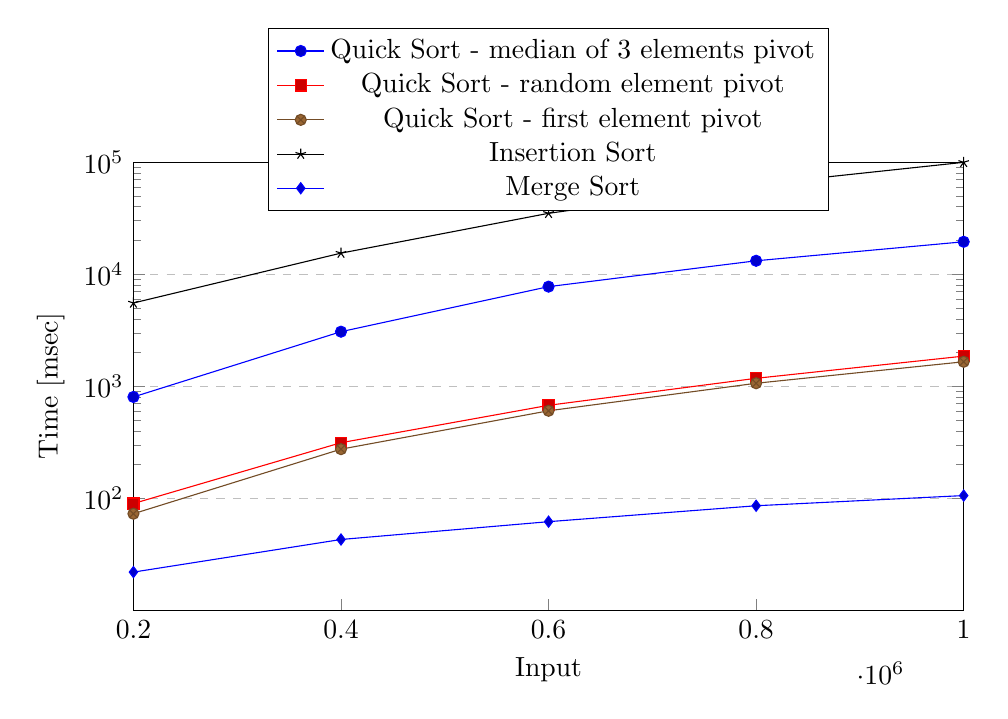
\begin{tikzpicture}
\begin{axis}[
    %title={Running times},
    width=1.0\textwidth,
    height=0.6\textwidth,
    xmode=normal,
    ymode=log,
    xlabel={Input},
    ylabel={Time [msec]},
    xmin=200000, xmax=1000000,
    ymin=10, ymax=100000,
    xtick={200000, 400000, 600000, 800000, 1000000},
    ytick={10e1, 10e2, 10e3, 10e4, 10e5},
    legend style={at={(0.5,1.3)},anchor=north},
    ymajorgrids=true,
    grid style=dashed]
\addplot
    coordinates {
    (200000,804)(400000,3073)(600000,7753)(800000,13186)(1000000,19487)
    };
\addlegendentry{Quick Sort - median of 3 elements pivot}
\addplot
    coordinates {
    (200000,90)(400000,314)(600000,677)(800000,1179)(1000000,1860)
    };
\addlegendentry{Quick Sort - random element pivot}
\addplot
    coordinates {
    (200000,73)(400000,275)(600000,605)(800000,1065)(1000000,1656)
    };
\addlegendentry{Quick Sort - first element pivot}
\addplot
    coordinates {
    (200000,5541)(400000,15428)(600000,34965)(800000,63185)(1000000,99659)
    };
\addlegendentry{Insertion Sort}
\addplot
    coordinates {
    (200000,22)(400000,43)(600000,62)(800000,86)(1000000,106)
    };
\addlegendentry{Merge Sort}
\addplot
    coordinates {
    (200000,0)(400000,0)(600000,0)(800000,0)(1000000,0)
    };
\addlegendentry{Binary Search}
\end{axis}
\end{tikzpicture}
\captionof{figure}{Running times of all the tested algorithms.}
\end{center}

\newpage
\section{Quick Sort}
\subsection{Median of 3 elements pivot}

\begin{center}
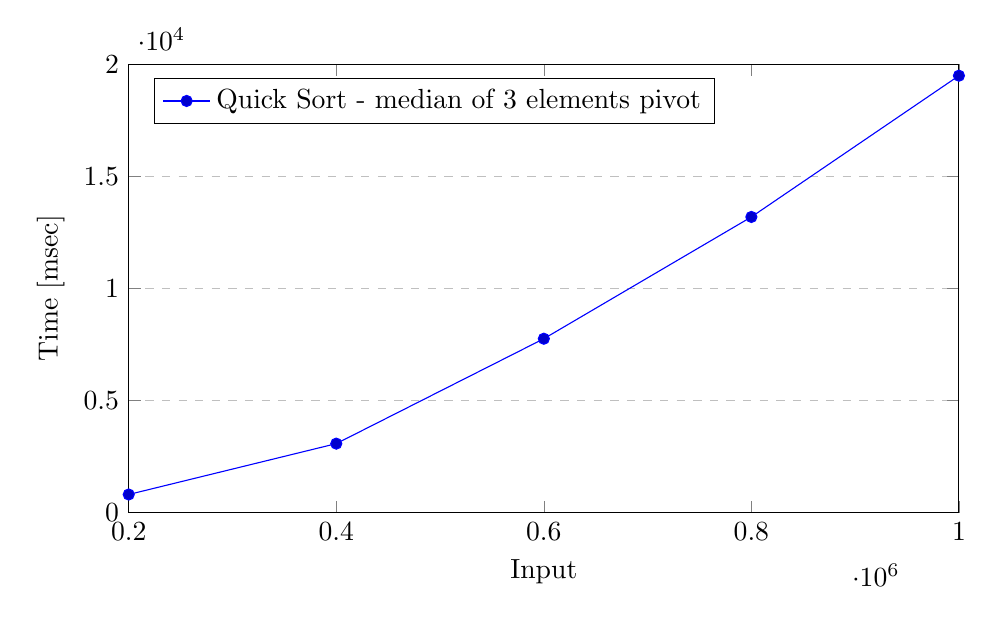
\begin{tikzpicture}
\begin{axis}[
    %title={Running times},
    width=1.0\textwidth,
    height=0.6\textwidth,
    xmode=normal,
    ymode=normal,
    xlabel={Input},
    ylabel={Time [msec]},
    xmin=200000, xmax=1000000,
    ymin=0, ymax=20000,
    xtick={200000, 400000, 600000, 800000, 1000000},
    ytick=,
    legend pos=north west,
    ymajorgrids=true,
    grid style=dashed,
    legend pos=north west]
\addplot
    coordinates {
    (200000,804)(400000,3073)(600000,7753)(800000,13186)(1000000,19487)
    };
\addlegendentry{Quick Sort - median of 3 elements pivot}
% \addplot [
%     domain=200000:1000000, 
%     samples=100, 
%     ]
%     {0.00019875*x*(log2(x))};
\end{axis}
\end{tikzpicture}
\captionof{figure}{Running times of Quick Sort - Median of 3 elements pivot.}
\end{center}

\textbf{Computation on T(N)}\\

Expected complexity: $O(NlogN)$\\

\LOG[2]{2}{\logTwoResult}
\MULTIPLY{\logTwoResult}{2}{\logTwoMultiplied}
\LOG[2]{10}{\logTenResult}
\MULTIPLY{\logTenResult}{10}{\logTenMultiplied}

\begin{enumerate}
    \MULTIPLY{804}{\logTwoMultiplied}{\resultQuickSortMedianTwoTimes}
    \item $T(400\,000) = 804 *2 log 2 = \resultQuickSortMedianTwoTimes < 3073$\\
    The algorithm is twice as fast as the worst case.
    
    % \MULTIPLY{804}{\logTenMultiplied}{\resultQuickSortMedianTenTimes}
    \item $T(1\,000\,000) = 804 *10 log 10 =$
    % \directlua{tex.print(math.floor(804*10*math.log(10, 2)))}
    $> 19487$\\
    The algorithm is slower than the theoretical worst case.
    
\end{enumerate}

\textbf{Analysis}\\

In theory this algorithm should have been the fastest implementation of QuickSort but probably due to its recursive implementation turned out to be the slowest. Recursion is usually slower than iteration because the CPU has to deal with the recursive call stack frame, in addition to processing the loop content.

\newpage
\subsection{Random element pivot}

\begin{center}
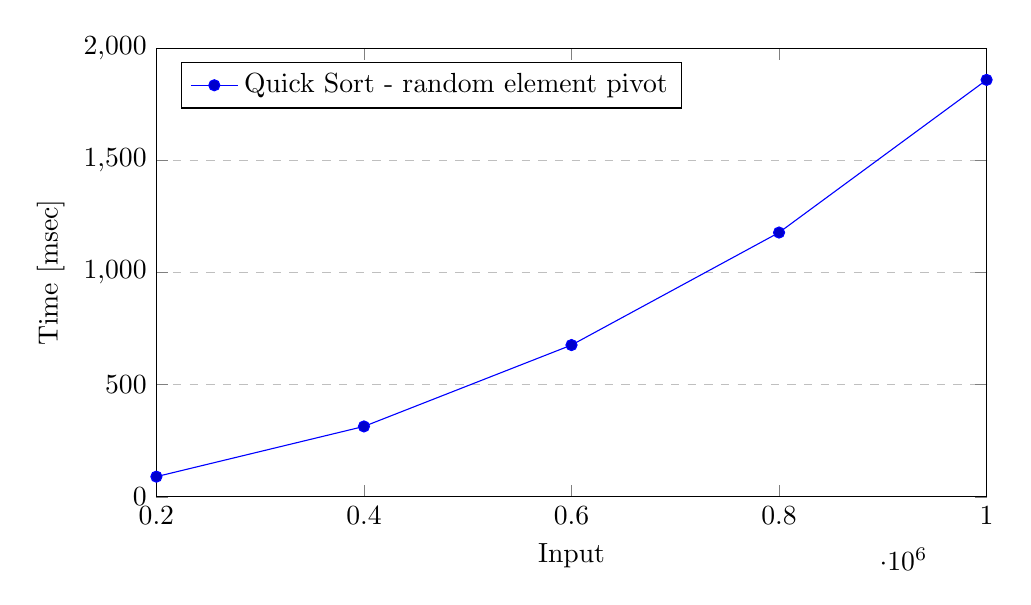
\begin{tikzpicture}
\begin{axis}[
    %title={Running times},
    width=1.0\textwidth,
    height=0.6\textwidth,
    xmode=normal,
    ymode=normal,
    xlabel={Input},
    ylabel={Time [msec]},
    xmin=200000, xmax=1000000,
    ymin=0, ymax=2000,
    xtick={200000, 400000, 600000, 800000, 1000000},
    ytick=,
    legend pos=north west,
    ymajorgrids=true,
    grid style=dashed,
    legend pos=north west]
\addplot
    coordinates {
    (200000,90)(400000,314)(600000,677)(800000,1179)(1000000,1860)
    };
\addlegendentry{Quick Sort - random element pivot}
\end{axis}
\end{tikzpicture}
\captionof{figure}{Running times of Quick Sort - Random element pivot.}
\end{center}

\textbf{Computation on T(N)}\\

Expected complexity: $O(NlogN)$\\

\begin{enumerate}
    \item $T(400\,000) = 90 *2 log 2 =$
    % \directlua{tex.print(math.floor(90*2*math.log(2, 2)))}
    $< 314$\\
    The algorithm is almost twice as fast as the worst case.
    
    % \MULTIPLY{804}{\logTenMultiplied}{\resultQuickSortMedianTenTimes}
    \item $T(1\,000\,000) = 90 *10 log 10 =$
    % \directlua{tex.print(math.floor(90*10*math.log(10, 2)))}
    $> 1860$\\
    The algorithm is slower than the theoretical worst case.
    
\end{enumerate}

\newpage
\subsection{First element pivot}

\begin{center}
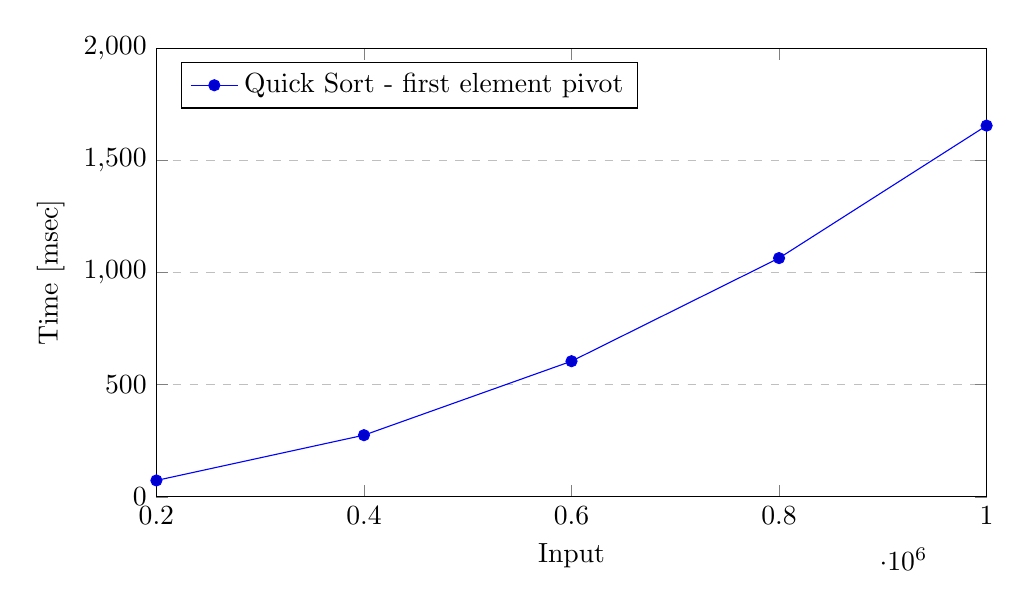
\begin{tikzpicture}
\begin{axis}[
    %title={Running times},
    width=1.0\textwidth,
    height=0.6\textwidth,
    xmode=normal,
    ymode=normal,
    xlabel={Input},
    ylabel={Time [msec]},
    xmin=200000, xmax=1000000,
    ymin=0, ymax=2000,
    xtick={200000, 400000, 600000, 800000, 1000000},
    ytick=,
    legend pos=north west,
    ymajorgrids=true,
    grid style=dashed,
    legend pos=north west]
\addplot
    coordinates {
    (200000,73)(400000,275)(600000,605)(800000,1065)(1000000,1656)
    };
\addlegendentry{Quick Sort - first element pivot}
\end{axis}
\end{tikzpicture}
\captionof{figure}{Running times of Quick Sort - First element pivot.}
\end{center}

\textbf{Computation on T(N)}\\

Expected complexity: $O(NlogN)$\\

\begin{enumerate}
    \item $T(400\,000) = 73 *2 log 2 =$
    % \directlua{tex.print(math.floor(73*2*math.log(2, 2)))}
    $< 275$\\
    The algorithm is twice as fast as the worst case.
    
    % \MULTIPLY{804}{\logTenMultiplied}{\resultQuickSortMedianTenTimes}
    \item $T(1\,000\,000) = 73 *10 log 10 =$
    % \directlua{tex.print(math.floor(73*10*math.log(10, 2)))}
    $> 1656$\\
    The algorithm is slower than the theoretical worst case.
    
\end{enumerate}

\textbf{Analysis}\\

The performance of this algorithm are extremely similar to that of QuickSort with a random element pivot. This is partially expected because both algorithm have a similar way of selecting the pivot even if one is implement in a recursive fashion and the other is iterative.

\newpage
\section{Insertion Sort}

\begin{center}
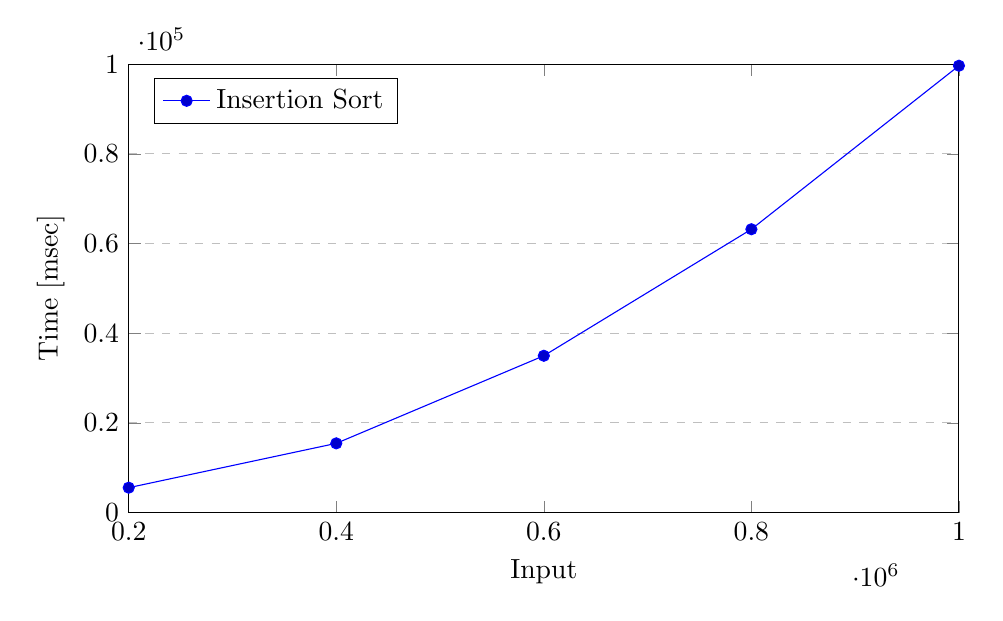
\begin{tikzpicture}
\begin{axis}[
    %title={Running times},
    width=1.0\textwidth,
    height=0.6\textwidth,
    xmode=normal,
    ymode=normal,
    xlabel={Input},
    ylabel={Time [msec]},
    xmin=200000, xmax=1000000,
    ymin=0, ymax=100000,
    xtick={200000, 400000, 600000, 800000, 1000000},
    ytick=,
    legend pos=north west,
    ymajorgrids=true,
    grid style=dashed,
    legend pos=north west]
\addplot
    coordinates {
    (200000,5541)(400000,15428)(600000,34965)(800000,63185)(1000000,99659)
    };
\addlegendentry{Insertion Sort}
\end{axis}
\end{tikzpicture}
\captionof{figure}{Running times of Insertion Sort.}
\end{center}

\textbf{Computation on T(N)}\\

Expected complexity: $O(N^2)$\\

\begin{enumerate}
    \item $T(400\,000) = 5541 *2^2 =$
    % \directlua{tex.print(math.floor(5541*2*2))}
    $> 15428$\\
    The algorithm is slower than the worst case.
    
    % \MULTIPLY{804}{\logTenMultiplied}{\resultQuickSortMedianTenTimes}
    \item $T(1\,000\,000) = 5541 *10^2 =$
    % \directlua{tex.print(math.floor(5541*10*10))}
    $> 99659$\\
    The algorithm is more than five time slower than the theoretical worst case.
    
\end{enumerate}

\textbf{Analysis}\\

As expected, Insertion Sort is the slowest algorithm  because it is better suited for small inputs or when data is nearly sorted which was not the case in this test.

\newpage
\section{Merge Sort}

\begin{center}
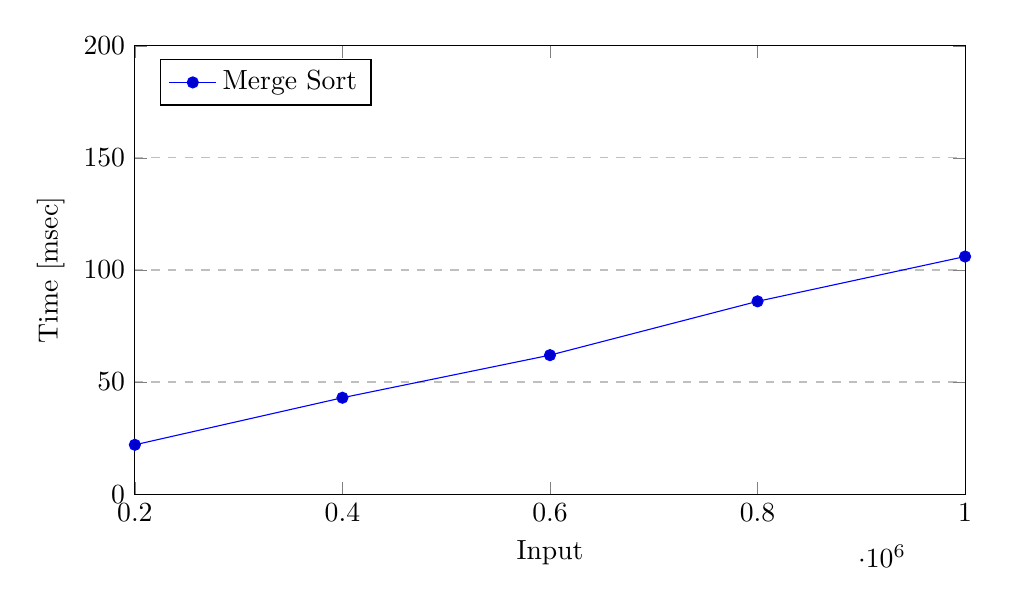
\begin{tikzpicture}
\begin{axis}[
    %title={Running times},
    width=1.0\textwidth,
    height=0.6\textwidth,
    xmode=normal,
    ymode=normal,
    xlabel={Input},
    ylabel={Time [msec]},
    xmin=200000, xmax=1000000,
    ymin=0, ymax=200,
    xtick={200000, 400000, 600000, 800000, 1000000},
    ytick=,
    legend pos=north west,
    ymajorgrids=true,
    grid style=dashed,
    legend pos=north west]
\addplot
    coordinates {
    (200000,22)(400000,43)(600000,62)(800000,86)(1000000,106)
    };
\addlegendentry{Merge Sort}
\end{axis}
\end{tikzpicture}
\captionof{figure}{Running times of Merge Sort.}
\end{center}

\textbf{Computation on T(N)}\\

Expected complexity: $O(NlogN)$\\

\begin{enumerate}
    \item $T(400\,000) = 22 *2 log 2 =$
    % \directlua{tex.print(math.floor(22*2*math.log(2, 2)))}
    $> 43$\\
    The algorithm execution time is nearly identical to the worst case.
    
    % \MULTIPLY{804}{\logTenMultiplied}{\resultQuickSortMedianTenTimes}
    \item $T(1\,000\,000) = 22 *10 log 10 =$
    % \directlua{tex.print(math.floor(22*10*math.log(10, 2)))}
    $> 106$\\
    The algorithm is slower than the theoretical worst case.
    
\end{enumerate}

\textbf{Analysis}\\

Merge Sort requires more memory space than Quick Sort but its recursive implementation is definitely the fastest.

\newpage
\section{Binary Search}

\begin{center}
\begin{tikzpicture}
\begin{axis}[
    %title={Running times},
    width=1.0\textwidth,
    height=0.6\textwidth,
    xmode=normal,
    ymode=normal,
    xlabel={Input},
    ylabel={Time [msec]},
    xmin=200000, xmax=1000000,
    ymin=0, ymax=10,
    xtick={200000, 400000, 600000, 800000, 1000000},
    ytick={},
    legend pos=north west,
    ymajorgrids=true,
    grid style=dashed,
    legend pos=north west]
\addplot
    coordinates {
    (200000,0)(400000,0)(600000,0)(800000,0)(1000000,0)
    };
\addlegendentry{Binary Search}
\end{axis}
\end{tikzpicture}
\captionof{figure}{Running times of Binary Search.}
\end{center}


\textbf{Computation on T(N)}\\

Expected complexity: $O(logN)$\\

\textbf{Analysis}\\

The implementation of Binary Search was so fast that for every input size the measured execution time was zero. Increasing the input size over 10 millions was not possible because of memory limitation on the PC used. It is nonetheless possible to conclude that its time complexity increase very slowly, most likely as predicted by the theory.

\newpage
\section{Conclusion}

Sorting algorithms are very important, useful and widely used so, finding the most efficient one for a given application can yield big benefits. Unfortunately theoretical analysis and practical implementations not always agrees thus, it is crucial to test the chosen algorithm before making a definitive choice. The specific use case and data structures that are going to be used can have a big impact on the final efficiency and mark a successful implementation from a failed one.

\newpage

\nocite{*}
\printbibliography[] % to hide showing references again

\end{document}
